\section*{Синтез 4х разрядного сдвигающего регистра}
\addcontentsline{toc}{section}{Синтез 4х разрядного сдвигающего регистра}
\subsection*{Аналитическая модель}
\addcontentsline{toc}{subsection}{Аналитическая модель}

Для построение 4х разрядного регистра потребуется 4 тригера. Исходя из этого
составим таблицу переходов тригера из состояния $Q_i^t$ в $Q_i^{t+1}$.

\begin{table}[h!]
    \centering
    \begin{tabular}{
        |>{\centering} m{0.5cm}
        |>{\centering} m{1.4cm}
        |>{\centering} m{1.4cm}
        |>{\centering} m{1.4cm}
        |>{\centering} m{1.4cm}
        |>{\centering} m{1.4cm}
        |>{\centering} m{1.4cm}
        |>{\centering} m{1.4cm}
        |>{\centering\arraybackslash} m{1.4cm} |
    }
        \hline
        № & $Q_1^t$ & $Q_2^t$ & $Q_3^t$ & $Q_4^t$ & $Q_1^{t+1}$ & $Q_2^{t+1}$ & $Q_3^{t+1}$ & $Q_4^{t+1}$\rowend
        1  & 0 & 0 & 0 & 0 & 0 & 0 & 0 & 0 \rowend
        2  & 0 & 0 & 0 & 1 & 0 & 0 & 0 & 0 \rowend
        3  & 0 & 0 & 1 & 0 & 0 & 0 & 0 & 1 \rowend
        4  & 0 & 0 & 1 & 1 & 0 & 0 & 0 & 1 \rowend
        5  & 0 & 1 & 0 & 0 & 0 & 0 & 1 & 0 \rowend
        6  & 0 & 1 & 0 & 1 & 0 & 0 & 1 & 0 \rowend
        7  & 0 & 1 & 1 & 0 & 0 & 0 & 1 & 1 \rowend
        8  & 0 & 1 & 1 & 1 & 0 & 0 & 1 & 1 \rowend
        9  & 1 & 0 & 0 & 0 & 0 & 1 & 0 & 0 \rowend
        10 & 1 & 0 & 0 & 1 & 0 & 1 & 0 & 0 \rowend
        11 & 1 & 0 & 1 & 0 & 0 & 1 & 0 & 1 \rowend
        12 & 1 & 0 & 1 & 1 & 0 & 1 & 0 & 1 \rowend
        13 & 1 & 1 & 0 & 0 & 0 & 1 & 1 & 0 \rowend
        14 & 1 & 1 & 0 & 1 & 0 & 1 & 1 & 0 \rowend
        15 & 1 & 1 & 1 & 0 & 0 & 1 & 1 & 1 \rowend
        16 & 1 & 1 & 1 & 1 & 0 & 1 & 1 & 1 \rowend
    \end{tabular}
    \caption{Таблица функционирования регистра}
\end{table}

На основании таблицы функционирования регистра были составлены прикладные
таблицы для каждого триггера регистра. Прикладные таблицы отражают
переход данного триггера из предыдущего состояния в последующее. Для составления
прикладных таблиц в клетки карты, соответствующие номерам предыдущих состояний
автомата, вписываются 2-разрядные двоичные числа, выражающие переход триггера при
изменении состояния автомата.

\begin{center}
    \begin{tabular}{
        |>\centering m{2cm}
        |>\centering m{0.9cm}
        |>\centering m{0.9cm}
        |>\centering m{0.9cm}
        |>\centering m{0.9cm}
        |>{\centering\arraybackslash} m{0.9cm} |
    }
        \hline
        $Q_1^t\rightarrow Q_1^{t+1}$ & $Q_3$ & $Q_3$ & $\overline{Q}_3$ & $\overline{Q}_3$ & \rowend
        $Q_4$            & 00 & 10 & 10 & 00 & $\overline{Q}_2$ \rowend
        $Q_4$            & 00 & 10 & 10 & 00 & $Q_2$ \rowend
        $\overline{Q}_4$ & 00 & 10 & 10 & 00 & $Q_2$ \rowend
        $\overline{Q}_4$ & 00 & 10 & 10 & 00 & $\overline{Q}_2$\rowend
         & $\overline{Q}_1$ & $Q_1$ & $Q_1$ & $\overline{Q}_1$ & \rowend
    \end{tabular}
    \captionof{table}{Прикладная таблица для $Q_1$}
\end{center}

\begin{center}
    \begin{tabular}{
        |>\centering m{2cm}
        |>\centering m{0.9cm}
        |>\centering m{0.9cm}
        |>\centering m{0.9cm}
        |>\centering m{0.9cm}
        |>{\centering\arraybackslash} m{0.9cm} |
    }
        \hline
        $Q_2^t\rightarrow Q_2^{t+1}$ & $Q_3$ & $Q_3$ & $\overline{Q}_3$ & $\overline{Q}_3$ & \rowend
        $Q_4$            & 00 & 01 & 01 & 00 & $\overline{Q}_2$ \rowend
        $Q_4$            & 10 & 11 & 11 & 10 & $Q_2$ \rowend
        $\overline{Q}_4$ & 10 & 11 & 11 & 10 & $Q_2$ \rowend
        $\overline{Q}_4$ & 00 & 01 & 01 & 00 & $\overline{Q}_2$\rowend
         & $\overline{Q}_1$ & $Q_1$ & $Q_1$ & $\overline{Q}_1$ & \rowend
    \end{tabular}
    \captionof{table}{Прикладная таблица для $Q_2$}
\end{center}

\begin{center}
    \begin{tabular}{
        |>\centering m{2cm}
        |>\centering m{0.9cm}
        |>\centering m{0.9cm}
        |>\centering m{0.9cm}
        |>\centering m{0.9cm}
        |>{\centering\arraybackslash} m{0.9cm} |
    }
        \hline
        $Q_3^t\rightarrow Q_3^{t+1}$ & $Q_3$ & $Q_3$ & $\overline{Q}_3$ & $\overline{Q}_3$ & \rowend
        $Q_4$            & 10 & 10 & 00 & 00 & $\overline{Q}_2$ \rowend
        $Q_4$            & 11 & 11 & 01 & 01 & $Q_2$ \rowend
        $\overline{Q}_4$ & 11 & 11 & 01 & 01 & $Q_2$ \rowend
        $\overline{Q}_4$ & 10 & 10 & 00 & 00 & $\overline{Q}_2$\rowend
         & $\overline{Q}_1$ & $Q_1$ & $Q_1$ & $\overline{Q}_1$ & \rowend
    \end{tabular}
    \captionof{table}{Прикладная таблица для $Q_3$}
\end{center}

\begin{center}
    \begin{tabular}{
        |>\centering m{2cm}
        |>\centering m{0.9cm}
        |>\centering m{0.9cm}
        |>\centering m{0.9cm}
        |>\centering m{0.9cm}
        |>{\centering\arraybackslash} m{0.9cm} |
    }
        \hline
        $Q_4^t\rightarrow Q_4^{t+1}$ & $Q_3$ & $Q_3$ & $\overline{Q}_3$ & $\overline{Q}_3$ & \rowend
        $Q_4$            & 11 & 11 & 10 & 10 & $\overline{Q}_2$ \rowend
        $Q_4$            & 11 & 11 & 10 & 10 & $Q_2$ \rowend
        $\overline{Q}_4$ & 01 & 01 & 00 & 00 & $Q_2$ \rowend
        $\overline{Q}_4$ & 01 & 01 & 00 & 00 & $\overline{Q}_2$\rowend
         & $\overline{Q}_1$ & $Q_1$ & $Q_1$ & $\overline{Q}_1$ & \rowend
    \end{tabular}
    \captionof{table}{Прикладная таблица для $Q_4$}
\end{center}

В качестве элементной базы были выбраны триггеры D типа, которые имеют следующую
характеристическую таблицу:


\begin{center}
    \begin{tabular}{
        |>\centering m{2cm}
        |>{\centering\arraybackslash} m{2cm} |
    }
        \hline
        $Q^t\rightarrow Q^{t+1}$ & $D^t$ \rowend
        00 & 0 \rowend
        01 & 1 \rowend
        10 & 0 \rowend
        11 & 1 \rowend
    \end{tabular}
    \captionof{table}{ Характеристическая таблица для триаггера типа D}
\end{center}

На основании полученных прикладных таблиц и характеристической таблицы D триггера
были составлены карты Карно для входов каждого триггера (Таблицы 7-10). Для этого
2-разрядные двоичные числа в прикладных таблицах были заменены соответствующими
обобщёнными значениями из клеток характеристической таблицы для каждого входа
триггера.

\begin{center}
    \begin{tabular}{
        |>\centering m{2cm}
        |>\centering m{0.9cm}
        |>\centering m{0.9cm}
        |>\centering m{0.9cm}
        |>\centering m{0.9cm}
        |>{\centering\arraybackslash} m{0.9cm} |
    }
        \hline
        $Q_1^t\rightarrow Q_1^{t+1}$ & $Q_3$ & $Q_3$ & $\overline{Q}_3$ & $\overline{Q}_3$ & \rowend
        $Q_4$            & 0 & 0 & 0 & 0 & $\overline{Q}_2$ \rowend
        $Q_4$            & 0 & 0 & 0 & 0 & $Q_2$ \rowend
        $\overline{Q}_4$ & 0 & 0 & 0 & 0 & $Q_2$ \rowend
        $\overline{Q}_4$ & 0 & 0 & 0 & 0 & $\overline{Q}_2$\rowend
         & $\overline{Q}_1$ & $Q_1$ & $Q_1$ & $\overline{Q}_1$ & \rowend
    \end{tabular}
    \captionof{table}{Карта Карно для $D_1$ входа}
\end{center}

\begin{center}
    \begin{tabular}{
        |>\centering m{2cm}
        |>\centering m{0.9cm}
        |>\centering m{0.9cm}
        |>\centering m{0.9cm}
        |>\centering m{0.9cm}
        |>{\centering\arraybackslash} m{0.9cm} |
    }
        \hline
        $Q_2^t\rightarrow Q_2^{t+1}$ & $Q_3$ & $Q_3$ & $\overline{Q}_3$ & $\overline{Q}_3$ & \rowend
        $Q_4$            & 0 & 1 & 1 & 0 & $\overline{Q}_2$ \rowend
        $Q_4$            & 0 & 1 & 1 & 0 & $Q_2$ \rowend
        $\overline{Q}_4$ & 0 & 1 & 1 & 0 & $Q_2$ \rowend
        $\overline{Q}_4$ & 0 & 1 & 1 & 0 & $\overline{Q}_2$\rowend
         & $\overline{Q}_1$ & $Q_1$ & $Q_1$ & $\overline{Q}_1$ & \rowend
    \end{tabular}
    \captionof{table}{Карта Карно для $D_2$ входа}
\end{center}

\begin{center}
    \begin{tabular}{
        |>\centering m{2cm}
        |>\centering m{0.9cm}
        |>\centering m{0.9cm}
        |>\centering m{0.9cm}
        |>\centering m{0.9cm}
        |>{\centering\arraybackslash} m{0.9cm} |
    }
        \hline
        $Q_3^t\rightarrow Q_3^{t+1}$ & $Q_3$ & $Q_3$ & $\overline{Q}_3$ & $\overline{Q}_3$ & \rowend
        $Q_4$            & 0 & 0 & 0 & 0 & $\overline{Q}_2$ \rowend
        $Q_4$            & 1 & 1 & 1 & 1 & $Q_2$ \rowend
        $\overline{Q}_4$ & 1 & 1 & 1 & 1 & $Q_2$ \rowend
        $\overline{Q}_4$ & 0 & 0 & 0 & 0 & $\overline{Q}_2$\rowend
         & $\overline{Q}_1$ & $Q_1$ & $Q_1$ & $\overline{Q}_1$ & \rowend
    \end{tabular}
    \captionof{table}{Карта Карно для $D_3$}
\end{center}

\begin{center}
    \begin{tabular}{
        |>\centering m{2cm}
        |>\centering m{0.9cm}
        |>\centering m{0.9cm}
        |>\centering m{0.9cm}
        |>\centering m{0.9cm}
        |>{\centering\arraybackslash} m{0.9cm} |
    }
        \hline
        $Q_4^t\rightarrow Q_4^{t+1}$ & $Q_3$ & $Q_3$ & $\overline{Q}_3$ & $\overline{Q}_3$ & \rowend
        $Q_4$            & 1 & 1 & 0 & 0 & $\overline{Q}_2$ \rowend
        $Q_4$            & 1 & 1 & 0 & 0 & $Q_2$ \rowend
        $\overline{Q}_4$ & 1 & 1 & 0 & 0 & $Q_2$ \rowend
        $\overline{Q}_4$ & 1 & 1 & 0 & 0 & $\overline{Q}_2$\rowend
         & $\overline{Q}_1$ & $Q_1$ & $Q_1$ & $\overline{Q}_1$ & \rowend
    \end{tabular}
    \captionof{table}{Карта Карно для $D_4$ входа}
\end{center}

В результате был получен набор карт Карно, отражающих значения логических функций
на входах каждого триггера в зависимости от состояний счётчика.
Из полученного набора карт Карно были составлены логические уравнения входов
триггеров, которые связывают между собой входы и выходы всех триггеров счётчика:

$$
    D_1=0; D_2=Q_1; D_3=Q_2; D_4=Q_3;
$$

\newpage

\subsection*{Построение модели в Multisim}
\addcontentsline{toc}{subsection}{Построение модели в Multisim}

По полученным уравнениям был в Multisim был построен требуемый регистр.
Ко входу D был подключен ключ, а на входы CLK тригеров был подключен генератор
сигнала для более наглядной симуляции сдвига.

\begin{figure}[h!]
    \centering
    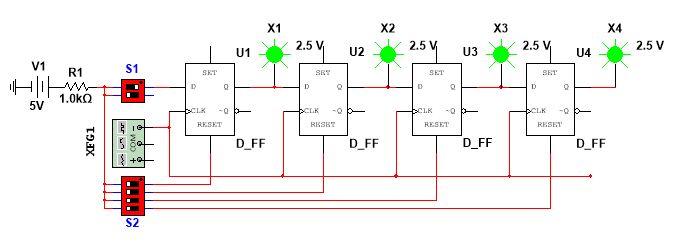
\includegraphics[scale=0.9]{images/image-1.png}
    \captionof{figure}{4х разрядный сдвигающий триггер}
\end{figure}



